Пояснения к примеру.

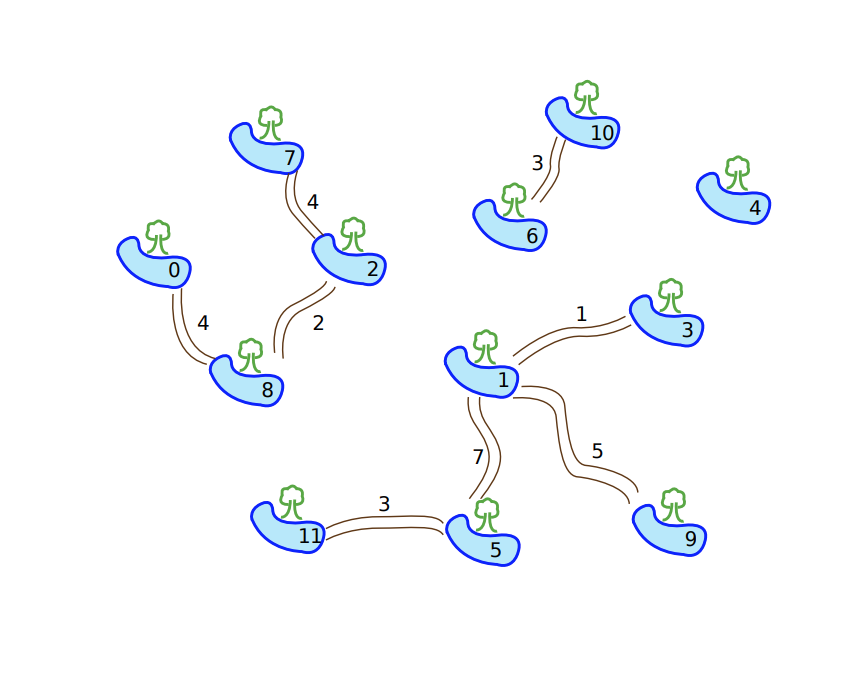
\includegraphics{dreaming1.png}

На рисунке выше показаны $N = 12$ озёр и $M = 8$ изначально заданных тропинок.
Предположим, что $L = 2$, то есть время перемещения по каждой из новых тропинок
занимает $2$ дня. Тогда Кенгуру может построить такие три новых тропинки:
\begin{itemize}
\item между озёрами $1$ и $2$;
\item между озёрами $1$ и $6$;
\item между озёрами $4$ и $10$.
\end{itemize}

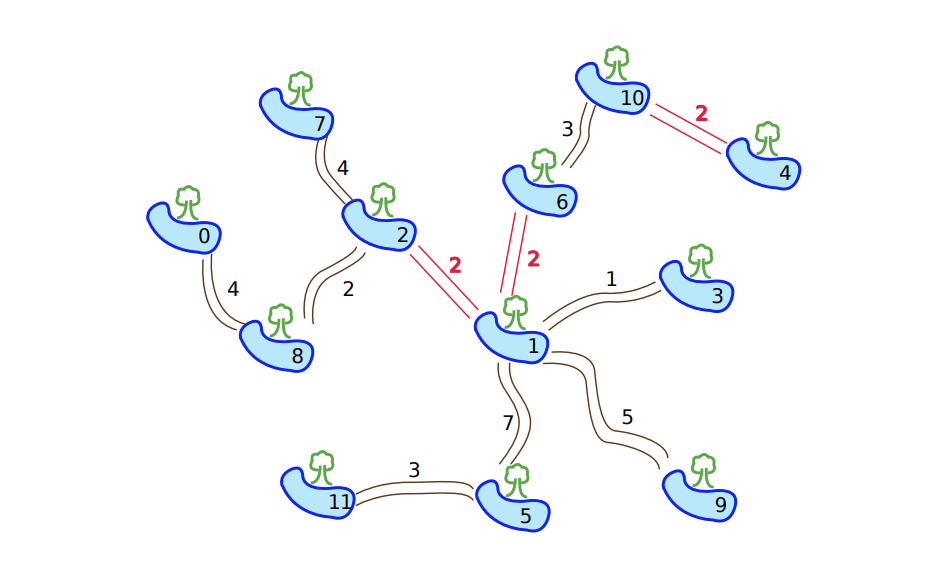
\includegraphics{dreaming2.png}

На рисунке выше показан окончательный набор тропинок. Максимальное время
путешествия~--- $18$ дней, оно достигается при путешествии между озёрами $0$ и $11$. Это
наименьшее возможное максимальное время путешествия: как бы Кенгуру ни строил
новые тропинки, всегда будет находиться какая­то пара озёр, для путешествия между
которыми потребуется $18$ дней или более.

Ваша программа должна содержать \t{\#include "dreaming.h"}.